\documentclass[1p]{elsarticle_modified}
%\bibliographystyle{elsarticle-num}

%\usepackage[colorlinks]{hyperref}
%\usepackage{abbrmath_seonhwa} %\Abb, \Ascr, \Acal ,\Abf, \Afrak
\usepackage{amsfonts}
\usepackage{amssymb}
\usepackage{amsmath}
\usepackage{amsthm}
\usepackage{scalefnt}
\usepackage{amsbsy}
\usepackage{kotex}
\usepackage{caption}
\usepackage{subfig}
\usepackage{color}
\usepackage{graphicx}
\usepackage{xcolor} %% white, black, red, green, blue, cyan, magenta, yellow
\usepackage{float}
\usepackage{setspace}
\usepackage{hyperref}

\usepackage{tikz}
\usetikzlibrary{arrows}

\usepackage{multirow}
\usepackage{array} % fixed length table
\usepackage{hhline}

%%%%%%%%%%%%%%%%%%%%%
\makeatletter
\renewcommand*\env@matrix[1][\arraystretch]{%
	\edef\arraystretch{#1}%
	\hskip -\arraycolsep
	\let\@ifnextchar\new@ifnextchar
	\array{*\c@MaxMatrixCols c}}
\makeatother %https://tex.stackexchange.com/questions/14071/how-can-i-increase-the-line-spacing-in-a-matrix
%%%%%%%%%%%%%%%

\usepackage[normalem]{ulem}

\newcommand{\msout}[1]{\ifmmode\text{\sout{\ensuremath{#1}}}\else\sout{#1}\fi}
%SOURCE: \msout is \stkout macro in https://tex.stackexchange.com/questions/20609/strikeout-in-math-mode

\newcommand{\cancel}[1]{
	\ifmmode
	{\color{red}\msout{#1}}
	\else
	{\color{red}\sout{#1}}
	\fi
}

\newcommand{\add}[1]{
	{\color{blue}\uwave{#1}}
}

\newcommand{\replace}[2]{
	\ifmmode
	{\color{red}\msout{#1}}{\color{blue}\uwave{#2}}
	\else
	{\color{red}\sout{#1}}{\color{blue}\uwave{#2}}
	\fi
}

\newcommand{\Sol}{\mathcal{S}} %segment
\newcommand{\D}{D} %diagram
\newcommand{\A}{\mathcal{A}} %arc


%%%%%%%%%%%%%%%%%%%%%%%%%%%%%5 test

\def\sl{\operatorname{\textup{SL}}(2,\Cbb)}
\def\psl{\operatorname{\textup{PSL}}(2,\Cbb)}
\def\quan{\mkern 1mu \triangleright \mkern 1mu}

\theoremstyle{definition}
\newtheorem{thm}{Theorem}[section]
\newtheorem{prop}[thm]{Proposition}
\newtheorem{lem}[thm]{Lemma}
\newtheorem{ques}[thm]{Question}
\newtheorem{cor}[thm]{Corollary}
\newtheorem{defn}[thm]{Definition}
\newtheorem{exam}[thm]{Example}
\newtheorem{rmk}[thm]{Remark}
\newtheorem{alg}[thm]{Algorithm}

\newcommand{\I}{\sqrt{-1}}
\begin{document}

%\begin{frontmatter}
%
%\title{Boundary parabolic representations of knots up to 8 crossings}
%
%%% Group authors per affiliation:
%\author{Yunhi Cho} 
%\address{Department of Mathematics, University of Seoul, Seoul, Korea}
%\ead{yhcho@uos.ac.kr}
%
%
%\author{Seonhwa Kim} %\fnref{s_kim}}
%\address{Center for Geometry and Physics, Institute for Basic Science, Pohang, 37673, Korea}
%\ead{ryeona17@ibs.re.kr}
%
%\author{Hyuk Kim}
%\address{Department of Mathematical Sciences, Seoul National University, Seoul 08826, Korea}
%\ead{hyukkim@snu.ac.kr}
%
%\author{Seokbeom Yoon}
%\address{Department of Mathematical Sciences, Seoul National University, Seoul, 08826,  Korea}
%\ead{sbyoon15@snu.ac.kr}
%
%\begin{abstract}
%We find all boundary parabolic representation of knots up to 8 crossings.
%
%\end{abstract}
%\begin{keyword}
%    \MSC[2010] 57M25 
%\end{keyword}
%
%\end{frontmatter}

%\linenumbers
%\tableofcontents
%
\newcommand\colored[1]{\textcolor{white}{\rule[-0.35ex]{0.8em}{1.4ex}}\kern-0.8em\color{red} #1}%
%\newcommand\colored[1]{\textcolor{white}{ #1}\kern-2.17ex	\textcolor{white}{ #1}\kern-1.81ex	\textcolor{white}{ #1}\kern-2.15ex\color{red}#1	}

{\Large $\underline{11a_{186}~(K11a_{186})}$}

\setlength{\tabcolsep}{10pt}
\renewcommand{\arraystretch}{1.6}
\vspace{1cm}\begin{tabular}{m{100pt}>{\centering\arraybackslash}m{274pt}}
\multirow{5}{120pt}{
	\centering
	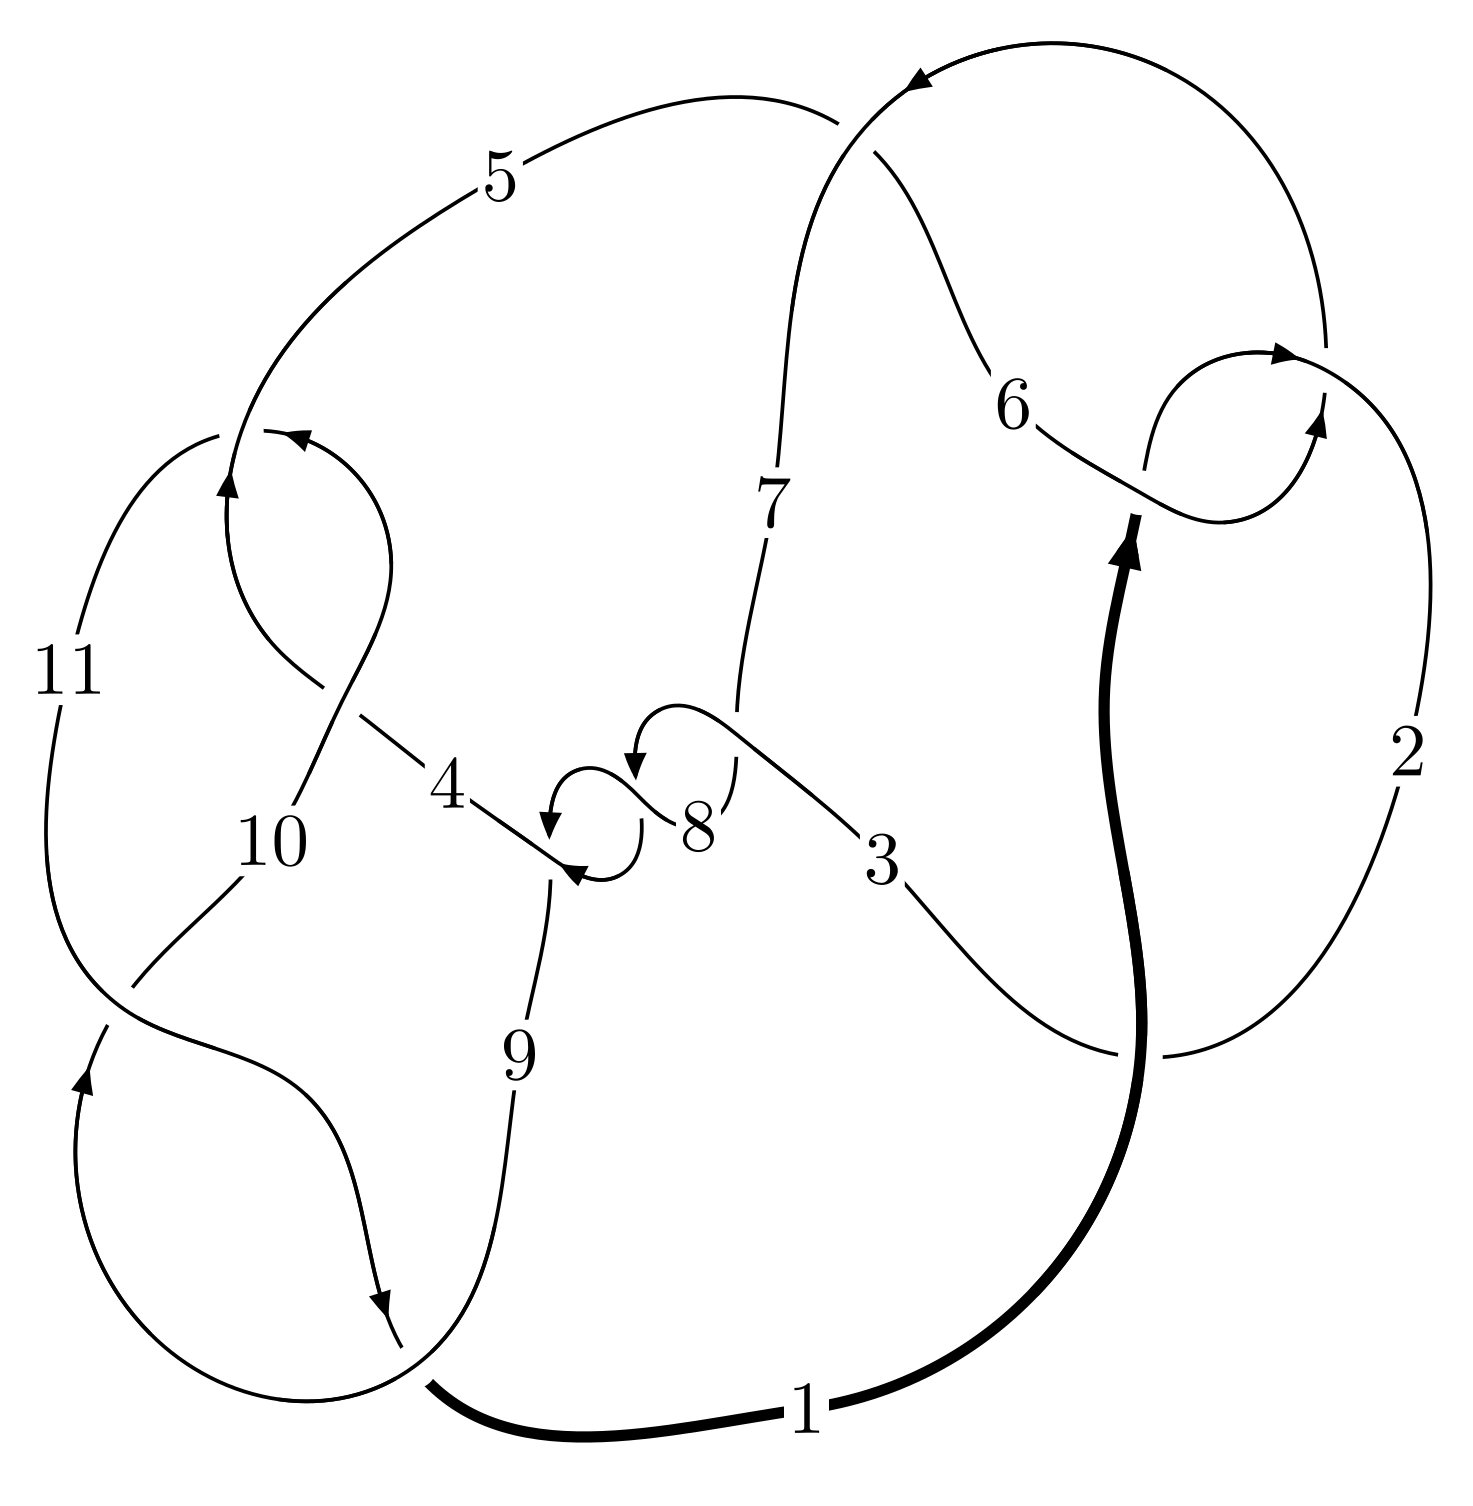
\includegraphics[width=112pt]{../../../GIT/diagram.site/Diagrams/png/435_11a_186.png}\\
\ \ \ A knot diagram\footnotemark}&
\allowdisplaybreaks
\textbf{Linearized knot diagam} \\
\cline{2-2}
 &
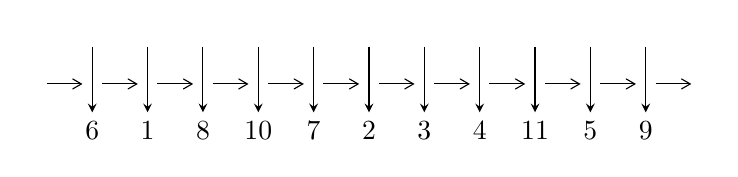
\begin{tikzpicture}[x=20pt, y=17pt]
	% nodes
	\node (C0) at (0, 0) {};
	\node (C1) at (1, 0) {};
	\node (C1U) at (1, +1) {};
	\node (C1D) at (1, -1) {6};

	\node (C2) at (2, 0) {};
	\node (C2U) at (2, +1) {};
	\node (C2D) at (2, -1) {1};

	\node (C3) at (3, 0) {};
	\node (C3U) at (3, +1) {};
	\node (C3D) at (3, -1) {8};

	\node (C4) at (4, 0) {};
	\node (C4U) at (4, +1) {};
	\node (C4D) at (4, -1) {10};

	\node (C5) at (5, 0) {};
	\node (C5U) at (5, +1) {};
	\node (C5D) at (5, -1) {7};

	\node (C6) at (6, 0) {};
	\node (C6U) at (6, +1) {};
	\node (C6D) at (6, -1) {2};

	\node (C7) at (7, 0) {};
	\node (C7U) at (7, +1) {};
	\node (C7D) at (7, -1) {3};

	\node (C8) at (8, 0) {};
	\node (C8U) at (8, +1) {};
	\node (C8D) at (8, -1) {4};

	\node (C9) at (9, 0) {};
	\node (C9U) at (9, +1) {};
	\node (C9D) at (9, -1) {11};

	\node (C10) at (10, 0) {};
	\node (C10U) at (10, +1) {};
	\node (C10D) at (10, -1) {5};

	\node (C11) at (11, 0) {};
	\node (C11U) at (11, +1) {};
	\node (C11D) at (11, -1) {9};
	\node (C12) at (12, 0) {};

	% arrows
	\draw[->,>={angle 60}]
	(C0) edge (C1) (C1) edge (C2) (C2) edge (C3) (C3) edge (C4) (C4) edge (C5) (C5) edge (C6) (C6) edge (C7) (C7) edge (C8) (C8) edge (C9) (C9) edge (C10) (C10) edge (C11) (C11) edge (C12) ;	\draw[->,>=stealth]
	(C1U) edge (C1D) (C2U) edge (C2D) (C3U) edge (C3D) (C4U) edge (C4D) (C5U) edge (C5D) (C6U) edge (C6D) (C7U) edge (C7D) (C8U) edge (C8D) (C9U) edge (C9D) (C10U) edge (C10D) (C11U) edge (C11D) ;
	\end{tikzpicture} \\
\hhline{~~} \\& 
\textbf{Solving Sequence} \\ \cline{2-2} 
 &
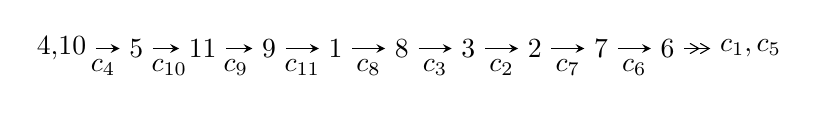
\begin{tikzpicture}[x=24pt, y=7pt]
	% node
	\node (A0) at (-1/8, 0) {4,10};
	\node (A1) at (1, 0) {5};
	\node (A2) at (2, 0) {11};
	\node (A3) at (3, 0) {9};
	\node (A4) at (4, 0) {1};
	\node (A5) at (5, 0) {8};
	\node (A6) at (6, 0) {3};
	\node (A7) at (7, 0) {2};
	\node (A8) at (8, 0) {7};
	\node (A9) at (9, 0) {6};
	\node (C1) at (1/2, -1) {$c_{4}$};
	\node (C2) at (3/2, -1) {$c_{10}$};
	\node (C3) at (5/2, -1) {$c_{9}$};
	\node (C4) at (7/2, -1) {$c_{11}$};
	\node (C5) at (9/2, -1) {$c_{8}$};
	\node (C6) at (11/2, -1) {$c_{3}$};
	\node (C7) at (13/2, -1) {$c_{2}$};
	\node (C8) at (15/2, -1) {$c_{7}$};
	\node (C9) at (17/2, -1) {$c_{6}$};
	\node (A10) at (41/4, 0) {$c_{1},c_{5}$};

	% edge
	\draw[->,>=stealth]	
	(A0) edge (A1) (A1) edge (A2) (A2) edge (A3) (A3) edge (A4) (A4) edge (A5) (A5) edge (A6) (A6) edge (A7) (A7) edge (A8) (A8) edge (A9) ;
	\draw[->>,>={angle 60}]	
	(A9) edge (A10);
\end{tikzpicture} \\ 

\end{tabular} \\

\footnotetext{
The image of knot diagram is generated by the software ``\textbf{Draw programme}" developed by Andrew Bartholomew(\url{http://www.layer8.co.uk/maths/draw/index.htm\#Running-draw}), where we modified some parts for our purpose(\url{https://github.com/CATsTAILs/LinksPainter}).
}\phantom \\ \newline 
\centering \textbf{Ideals for irreducible components\footnotemark of $X_{\text{par}}$} 
 
\begin{align*}
I^u_{1}&=\langle 
u^{11}-2 u^9+4 u^7- u^6-4 u^5+u^4+3 u^3-2 u^2-2 u+1\rangle \\
I^u_{2}&=\langle 
u^{36}+u^{35}+\cdots+u^3+1\rangle \\
\\
\end{align*}
\raggedright * 2 irreducible components of $\dim_{\mathbb{C}}=0$, with total 47 representations.\\
\footnotetext{All coefficients of polynomials are rational numbers. But the coefficients are sometimes approximated in decimal forms when there is not enough margin.}
\newpage
\renewcommand{\arraystretch}{1}
\centering \section*{I. $I^u_{1}= \langle u^{11}-2 u^9+4 u^7- u^6-4 u^5+u^4+3 u^3-2 u^2-2 u+1 \rangle$}
\flushleft \textbf{(i) Arc colorings}\\
\begin{tabular}{m{7pt} m{180pt} m{7pt} m{180pt} }
\flushright $a_{4}=$&$\begin{pmatrix}1\\0\end{pmatrix}$ \\
\flushright $a_{10}=$&$\begin{pmatrix}0\\u\end{pmatrix}$ \\
\flushright $a_{5}=$&$\begin{pmatrix}1\\u^2\end{pmatrix}$ \\
\flushright $a_{11}=$&$\begin{pmatrix}- u\\- u^3+u\end{pmatrix}$ \\
\flushright $a_{9}=$&$\begin{pmatrix}u^3\\u^5- u^3+u\end{pmatrix}$ \\
\flushright $a_{1}=$&$\begin{pmatrix}- u^5- u\\- u^7+u^5-2 u^3+u\end{pmatrix}$ \\
\flushright $a_{8}=$&$\begin{pmatrix}u^5+u\\u^5- u^3+u\end{pmatrix}$ \\
\flushright $a_{3}=$&$\begin{pmatrix}- u^{10}+u^8-2 u^6+u^4- u^2+1\\- u^{10}+2 u^8-3 u^6+2 u^4- u^2\end{pmatrix}$ \\
\flushright $a_{2}=$&$\begin{pmatrix}- u^{10}+u^8+u^7-2 u^6+u^4+u^3- u^2+1\\- u^{10}+u^9+2 u^8- u^7-3 u^6+2 u^5+2 u^4- u^3- u^2\end{pmatrix}$ \\
\flushright $a_{7}=$&$\begin{pmatrix}- u^{10}+u^8- u^7-2 u^6+2 u^5+u^4-2 u^3+2 u\\- u^{10}- u^9+2 u^8+u^7-3 u^6- u^5+3 u^4- u^2+u\end{pmatrix}$ \\
\flushright $a_{6}=$&$\begin{pmatrix}- u^{10}- u^9+2 u^8+u^7-3 u^6- u^5+3 u^4-2 u^2+u+1\\- u^9+u^8+2 u^7-2 u^6-3 u^5+3 u^4+2 u^3-3 u^2- u+1\end{pmatrix}$\\ \flushright $a_{6}=$&$\begin{pmatrix}- u^{10}- u^9+2 u^8+u^7-3 u^6- u^5+3 u^4-2 u^2+u+1\\- u^9+u^8+2 u^7-2 u^6-3 u^5+3 u^4+2 u^3-3 u^2- u+1\end{pmatrix}$\\&\end{tabular}
\flushleft \textbf{(ii) Obstruction class $= -1$}\\~\\
\flushleft \textbf{(iii) Cusp Shapes $= 4 u^9-4 u^8-8 u^7+4 u^6+12 u^5-12 u^4-8 u^3+8 u^2+4 u-18$}\\~\\
\newpage\renewcommand{\arraystretch}{1}
\flushleft \textbf{(iv) u-Polynomials at the component}\newline \\
\begin{tabular}{m{50pt}|m{274pt}}
Crossings & \hspace{64pt}u-Polynomials at each crossing \\
\hline $$\begin{aligned}c_{1},c_{4},c_{6}\\c_{10}\end{aligned}$$&$\begin{aligned}
&u^{11}-2 u^9+4 u^7+u^6-4 u^5- u^4+3 u^3+2 u^2-2 u-1
\end{aligned}$\\
\hline $$\begin{aligned}c_{2},c_{5},c_{9}\\c_{11}\end{aligned}$$&$\begin{aligned}
&u^{11}+4 u^{10}+\cdots+8 u+1
\end{aligned}$\\
\hline $$\begin{aligned}c_{3},c_{7},c_{8}\end{aligned}$$&$\begin{aligned}
&u^{11}+5 u^{10}+8 u^9+5 u^8+9 u^7+19 u^6+8 u^5-2 u^4+9 u^3+u^2-12 u-4
\end{aligned}$\\
\hline
\end{tabular}\\~\\
\newpage\renewcommand{\arraystretch}{1}
\flushleft \textbf{(v) Riley Polynomials at the component}\newline \\
\begin{tabular}{m{50pt}|m{274pt}}
Crossings & \hspace{64pt}Riley Polynomials at each crossing \\
\hline $$\begin{aligned}c_{1},c_{4},c_{6}\\c_{10}\end{aligned}$$&$\begin{aligned}
&y^{11}-4 y^{10}+\cdots+8 y-1
\end{aligned}$\\
\hline $$\begin{aligned}c_{2},c_{5},c_{9}\\c_{11}\end{aligned}$$&$\begin{aligned}
&y^{11}+8 y^{10}+\cdots+28 y-1
\end{aligned}$\\
\hline $$\begin{aligned}c_{3},c_{7},c_{8}\end{aligned}$$&$\begin{aligned}
&y^{11}-9 y^{10}+\cdots+152 y-16
\end{aligned}$\\
\hline
\end{tabular}\\~\\
\newpage\flushleft \textbf{(vi) Complex Volumes and Cusp Shapes}
$$\begin{array}{c|c|c}  
\text{Solutions to }I^u_{1}& \I (\text{vol} + \sqrt{-1}CS) & \text{Cusp shape}\\
 \hline 
\begin{aligned}
u &= \phantom{-}0.574057 + 0.778762 I\end{aligned}
 & -0.32700 + 2.62828 I & -9.00950 - 0.39606 I \\ \hline\begin{aligned}
u &= \phantom{-}0.574057 - 0.778762 I\end{aligned}
 & -0.32700 - 2.62828 I & -9.00950 + 0.39606 I \\ \hline\begin{aligned}
u &= -0.786275 + 0.725485 I\end{aligned}
 & \phantom{-}5.13423 + 2.26440 I & -5.35075 - 2.78673 I \\ \hline\begin{aligned}
u &= -0.786275 - 0.725485 I\end{aligned}
 & \phantom{-}5.13423 - 2.26440 I & -5.35075 + 2.78673 I \\ \hline\begin{aligned}
u &= -0.903688\phantom{ +0.000000I}\end{aligned}
 & -4.12325\phantom{ +0.000000I} & -21.6840\phantom{ +0.000000I} \\ \hline\begin{aligned}
u &= \phantom{-}1.13447\phantom{ +0.000000I}\end{aligned}
 & -11.8669\phantom{ +0.000000I} & -21.5190\phantom{ +0.000000I} \\ \hline\begin{aligned}
u &= \phantom{-}0.937682 + 0.702007 I\end{aligned}
 & \phantom{-}4.20048 - 8.65870 I & -8.03545 + 9.01618 I \\ \hline\begin{aligned}
u &= \phantom{-}0.937682 - 0.702007 I\end{aligned}
 & \phantom{-}4.20048 + 8.65870 I & -8.03545 - 9.01618 I \\ \hline\begin{aligned}
u &= -1.053250 + 0.672906 I\end{aligned}
 & -3.16344 + 13.64350 I & -13.1560 - 9.4873 I \\ \hline\begin{aligned}
u &= -1.053250 - 0.672906 I\end{aligned}
 & -3.16344 - 13.64350 I & -13.1560 + 9.4873 I \\ \hline\begin{aligned}
u &= \phantom{-}0.424792\phantom{ +0.000000I}\end{aligned}
 & -0.633212\phantom{ +0.000000I} & -15.6940\phantom{ +0.000000I}\\
 \hline 
 \end{array}$$\newpage\newpage\renewcommand{\arraystretch}{1}
\centering \section*{II. $I^u_{2}= \langle u^{36}+u^{35}+\cdots+u^3+1 \rangle$}
\flushleft \textbf{(i) Arc colorings}\\
\begin{tabular}{m{7pt} m{180pt} m{7pt} m{180pt} }
\flushright $a_{4}=$&$\begin{pmatrix}1\\0\end{pmatrix}$ \\
\flushright $a_{10}=$&$\begin{pmatrix}0\\u\end{pmatrix}$ \\
\flushright $a_{5}=$&$\begin{pmatrix}1\\u^2\end{pmatrix}$ \\
\flushright $a_{11}=$&$\begin{pmatrix}- u\\- u^3+u\end{pmatrix}$ \\
\flushright $a_{9}=$&$\begin{pmatrix}u^3\\u^5- u^3+u\end{pmatrix}$ \\
\flushright $a_{1}=$&$\begin{pmatrix}- u^5- u\\- u^7+u^5-2 u^3+u\end{pmatrix}$ \\
\flushright $a_{8}=$&$\begin{pmatrix}u^5+u\\u^5- u^3+u\end{pmatrix}$ \\
\flushright $a_{3}=$&$\begin{pmatrix}- u^{10}+u^8-2 u^6+u^4- u^2+1\\- u^{10}+2 u^8-3 u^6+2 u^4- u^2\end{pmatrix}$ \\
\flushright $a_{2}=$&$\begin{pmatrix}u^{22}-3 u^{20}+\cdots-3 u^4+1\\u^{24}-4 u^{22}+\cdots+8 u^4-2 u^2\end{pmatrix}$ \\
\flushright $a_{7}=$&$\begin{pmatrix}- u^{15}+2 u^{13}-4 u^{11}+4 u^9-4 u^7+4 u^5-2 u^3+2 u\\- u^{15}+3 u^{13}-6 u^{11}+7 u^9-6 u^7+4 u^5-2 u^3+u\end{pmatrix}$ \\
\flushright $a_{6}=$&$\begin{pmatrix}- u^{32}+5 u^{30}+\cdots+2 u^2+1\\- u^{32}+6 u^{30}+\cdots-6 u^4+2 u^2\end{pmatrix}$\\ \flushright $a_{6}=$&$\begin{pmatrix}- u^{32}+5 u^{30}+\cdots+2 u^2+1\\- u^{32}+6 u^{30}+\cdots-6 u^4+2 u^2\end{pmatrix}$\\&\end{tabular}
\flushleft \textbf{(ii) Obstruction class $= -1$}\\~\\
\flushleft \textbf{(iii) Cusp Shapes $= 4 u^{32}-24 u^{30}+88 u^{28}-224 u^{26}+440 u^{24}-700 u^{22}+928 u^{20}-1060 u^{18}+4 u^{17}+1048 u^{16}-16 u^{15}-912 u^{14}+36 u^{13}+692 u^{12}-52 u^{11}-452 u^{10}+52 u^9+256 u^8-44 u^7-116 u^6+32 u^5+44 u^4-20 u^3-8 u^2+8 u-14$}\\~\\
\newpage\renewcommand{\arraystretch}{1}
\flushleft \textbf{(iv) u-Polynomials at the component}\newline \\
\begin{tabular}{m{50pt}|m{274pt}}
Crossings & \hspace{64pt}u-Polynomials at each crossing \\
\hline $$\begin{aligned}c_{1},c_{4},c_{6}\\c_{10}\end{aligned}$$&$\begin{aligned}
&u^{36}- u^{35}+\cdots- u^3+1
\end{aligned}$\\
\hline $$\begin{aligned}c_{2},c_{5},c_{9}\\c_{11}\end{aligned}$$&$\begin{aligned}
&u^{36}+13 u^{35}+\cdots-10 u^2+1
\end{aligned}$\\
\hline $$\begin{aligned}c_{3},c_{7},c_{8}\end{aligned}$$&$\begin{aligned}
&(u^{18}-2 u^{17}+\cdots+2 u+1)^{2}
\end{aligned}$\\
\hline
\end{tabular}\\~\\
\newpage\renewcommand{\arraystretch}{1}
\flushleft \textbf{(v) Riley Polynomials at the component}\newline \\
\begin{tabular}{m{50pt}|m{274pt}}
Crossings & \hspace{64pt}Riley Polynomials at each crossing \\
\hline $$\begin{aligned}c_{1},c_{4},c_{6}\\c_{10}\end{aligned}$$&$\begin{aligned}
&y^{36}-13 y^{35}+\cdots-10 y^2+1
\end{aligned}$\\
\hline $$\begin{aligned}c_{2},c_{5},c_{9}\\c_{11}\end{aligned}$$&$\begin{aligned}
&y^{36}+19 y^{35}+\cdots-20 y+1
\end{aligned}$\\
\hline $$\begin{aligned}c_{3},c_{7},c_{8}\end{aligned}$$&$\begin{aligned}
&(y^{18}-18 y^{17}+\cdots-10 y+1)^{2}
\end{aligned}$\\
\hline
\end{tabular}\\~\\
\newpage\flushleft \textbf{(vi) Complex Volumes and Cusp Shapes}
$$\begin{array}{c|c|c}  
\text{Solutions to }I^u_{2}& \I (\text{vol} + \sqrt{-1}CS) & \text{Cusp shape}\\
 \hline 
\begin{aligned}
u &= -0.568398 + 0.797612 I\end{aligned}
 & -1.72161 - 8.10595 I & -11.08535 + 5.00657 I \\ \hline\begin{aligned}
u &= -0.568398 - 0.797612 I\end{aligned}
 & -1.72161 + 8.10595 I & -11.08535 - 5.00657 I \\ \hline\begin{aligned}
u &= \phantom{-}0.759891 + 0.733182 I\end{aligned}
 & \phantom{-}4.73704 + 3.18642 I & -6.45994 - 3.31717 I \\ \hline\begin{aligned}
u &= \phantom{-}0.759891 - 0.733182 I\end{aligned}
 & \phantom{-}4.73704 - 3.18642 I & -6.45994 + 3.31717 I \\ \hline\begin{aligned}
u &= -0.527375 + 0.775874 I\end{aligned}
 & -6.14948 - 1.48503 I & -15.5689 + 0.3788 I \\ \hline\begin{aligned}
u &= -0.527375 - 0.775874 I\end{aligned}
 & -6.14948 + 1.48503 I & -15.5689 - 0.3788 I \\ \hline\begin{aligned}
u &= -0.853258 + 0.641261 I\end{aligned}
 & \phantom{-}1.83259 + 2.50180 I & -6.41929 - 3.81694 I \\ \hline\begin{aligned}
u &= -0.853258 - 0.641261 I\end{aligned}
 & \phantom{-}1.83259 - 2.50180 I & -6.41929 + 3.81694 I \\ \hline\begin{aligned}
u &= -0.898798 + 0.229050 I\end{aligned}
 & -0.88834 + 4.72205 I & -15.5195 - 7.2621 I \\ \hline\begin{aligned}
u &= -0.898798 - 0.229050 I\end{aligned}
 & -0.88834 - 4.72205 I & -15.5195 + 7.2621 I \\ \hline\begin{aligned}
u &= \phantom{-}0.720307 + 0.524101 I\end{aligned}
 & -0.218096 + 0.036628 I & -13.43748 - 0.95651 I \\ \hline\begin{aligned}
u &= \phantom{-}0.720307 - 0.524101 I\end{aligned}
 & -0.218096 - 0.036628 I & -13.43748 + 0.95651 I \\ \hline\begin{aligned}
u &= -1.115130 + 0.024468 I\end{aligned}
 & -6.14948 + 1.48503 I & -15.5689 - 0.3788 I \\ \hline\begin{aligned}
u &= -1.115130 - 0.024468 I\end{aligned}
 & -6.14948 - 1.48503 I & -15.5689 + 0.3788 I \\ \hline\begin{aligned}
u &= \phantom{-}0.936753 + 0.611605 I\end{aligned}
 & -0.88834 - 4.72205 I & -15.5195 + 7.2621 I \\ \hline\begin{aligned}
u &= \phantom{-}0.936753 - 0.611605 I\end{aligned}
 & -0.88834 + 4.72205 I & -15.5195 - 7.2621 I \\ \hline\begin{aligned}
u &= -0.475172 + 0.740129 I\end{aligned}
 & -2.30993 + 5.17624 I & -11.82231 - 5.02355 I \\ \hline\begin{aligned}
u &= -0.475172 - 0.740129 I\end{aligned}
 & -2.30993 - 5.17624 I & -11.82231 + 5.02355 I \\ \hline\begin{aligned}
u &= \phantom{-}0.510565 + 0.712216 I\end{aligned}
 & -0.822851\phantom{ +0.000000I} & -9.60076 + 0. I\phantom{ +0.000000I} \\ \hline\begin{aligned}
u &= \phantom{-}0.510565 - 0.712216 I\end{aligned}
 & -0.822851\phantom{ +0.000000I} & -9.60076 + 0. I\phantom{ +0.000000I} \\ \hline\begin{aligned}
u &= \phantom{-}1.129810 + 0.032613 I\end{aligned}
 & -7.69896 - 6.87816 I & -17.6593 + 5.1131 I \\ \hline\begin{aligned}
u &= \phantom{-}1.129810 - 0.032613 I\end{aligned}
 & -7.69896 + 6.87816 I & -17.6593 - 5.1131 I \\ \hline\begin{aligned}
u &= -0.917289 + 0.702643 I\end{aligned}
 & \phantom{-}4.73704 + 3.18642 I & -6.45994 - 3.31717 I \\ \hline\begin{aligned}
u &= -0.917289 - 0.702643 I\end{aligned}
 & \phantom{-}4.73704 - 3.18642 I & -6.45994 + 3.31717 I \\ \hline\begin{aligned}
u &= \phantom{-}0.772239 + 0.333861 I\end{aligned}
 & -0.218096 - 0.036628 I & -13.43748 + 0.95651 I \\ \hline\begin{aligned}
u &= \phantom{-}0.772239 - 0.333861 I\end{aligned}
 & -0.218096 + 0.036628 I & -13.43748 - 0.95651 I \\ \hline\begin{aligned}
u &= \phantom{-}1.038670 + 0.636561 I\end{aligned}
 & -2.30993 - 5.17624 I & -11.82231 + 5.02355 I \\ \hline\begin{aligned}
u &= \phantom{-}1.038670 - 0.636561 I\end{aligned}
 & -2.30993 + 5.17624 I & -11.82231 - 5.02355 I \\ \hline\begin{aligned}
u &= -1.051520 + 0.626704 I\end{aligned}
 & -3.95239\phantom{ +0.000000I} & -14.4550 + 0. I\phantom{ +0.000000I} \\ \hline\begin{aligned}
u &= -1.051520 - 0.626704 I\end{aligned}
 & -3.95239\phantom{ +0.000000I} & -14.4550 + 0. I\phantom{ +0.000000I}\\
 \hline 
 \end{array}$$\newpage$$\begin{array}{c|c|c}  
\text{Solutions to }I^u_{2}& \I (\text{vol} + \sqrt{-1}CS) & \text{Cusp shape}\\
 \hline 
\begin{aligned}
u &= \phantom{-}1.045370 + 0.669009 I\end{aligned}
 & -1.72161 - 8.10595 I & -11.08535 + 5.00657 I \\ \hline\begin{aligned}
u &= \phantom{-}1.045370 - 0.669009 I\end{aligned}
 & -1.72161 + 8.10595 I & -11.08535 - 5.00657 I \\ \hline\begin{aligned}
u &= -1.056180 + 0.652350 I\end{aligned}
 & -7.69896 + 6.87816 I & -17.6593 - 5.1131 I \\ \hline\begin{aligned}
u &= -1.056180 - 0.652350 I\end{aligned}
 & -7.69896 - 6.87816 I & -17.6593 + 5.1131 I \\ \hline\begin{aligned}
u &= \phantom{-}0.049508 + 0.478803 I\end{aligned}
 & \phantom{-}1.83259 - 2.50180 I & -6.41929 + 3.81694 I \\ \hline\begin{aligned}
u &= \phantom{-}0.049508 - 0.478803 I\end{aligned}
 & \phantom{-}1.83259 + 2.50180 I & -6.41929 - 3.81694 I\\
 \hline 
 \end{array}$$\newpage
\newpage\renewcommand{\arraystretch}{1}
\centering \section*{ III. u-Polynomials}
\begin{tabular}{m{50pt}|m{274pt}}
Crossings & \hspace{64pt}u-Polynomials at each crossing \\
\hline $$\begin{aligned}c_{1},c_{4},c_{6}\\c_{10}\end{aligned}$$&$\begin{aligned}
&(u^{11}-2 u^9+4 u^7+u^6-4 u^5- u^4+3 u^3+2 u^2-2 u-1)\\
&\cdot(u^{36}- u^{35}+\cdots- u^3+1)
\end{aligned}$\\
\hline $$\begin{aligned}c_{2},c_{5},c_{9}\\c_{11}\end{aligned}$$&$\begin{aligned}
&(u^{11}+4 u^{10}+\cdots+8 u+1)(u^{36}+13 u^{35}+\cdots-10 u^2+1)
\end{aligned}$\\
\hline $$\begin{aligned}c_{3},c_{7},c_{8}\end{aligned}$$&$\begin{aligned}
&(u^{11}+5 u^{10}+8 u^9+5 u^8+9 u^7+19 u^6+8 u^5-2 u^4+9 u^3+u^2-12 u-4)\\
&\cdot(u^{18}-2 u^{17}+\cdots+2 u+1)^{2}
\end{aligned}$\\
\hline
\end{tabular}\newpage\renewcommand{\arraystretch}{1}
\centering \section*{ IV. Riley Polynomials}
\begin{tabular}{m{50pt}|m{274pt}}
Crossings & \hspace{64pt}Riley Polynomials at each crossing \\
\hline $$\begin{aligned}c_{1},c_{4},c_{6}\\c_{10}\end{aligned}$$&$\begin{aligned}
&(y^{11}-4 y^{10}+\cdots+8 y-1)(y^{36}-13 y^{35}+\cdots-10 y^2+1)
\end{aligned}$\\
\hline $$\begin{aligned}c_{2},c_{5},c_{9}\\c_{11}\end{aligned}$$&$\begin{aligned}
&(y^{11}+8 y^{10}+\cdots+28 y-1)(y^{36}+19 y^{35}+\cdots-20 y+1)
\end{aligned}$\\
\hline $$\begin{aligned}c_{3},c_{7},c_{8}\end{aligned}$$&$\begin{aligned}
&(y^{11}-9 y^{10}+\cdots+152 y-16)(y^{18}-18 y^{17}+\cdots-10 y+1)^{2}
\end{aligned}$\\
\hline
\end{tabular}
\vskip 2pc
\end{document}